\chapter{Related work}
\label{cha:related-work}
This chapter discusses the related work researched while designing the NanoTorrent protocol. Section \ref{sec:related:internet} elaborates on \acrlong{P2P} protocols for the Internet like BitTorrent, whereas section \ref{sec:related:wsn} looks at protocols designed for \glspl{WSN}. As an exploration for a potential use case, section \ref{sec:related:evolution} looks at software evolution in \glspl{WSN}. Section \ref{sec:related:discussion} concludes with a critical discussion of the researched material.

\section{Peer-to-peer distribution for the Internet}
\label{sec:related:internet}

\subsection{BitTorrent}
\label{sec:related:bittorrent}
BitTorrent \cite{bep3} is a peer-to-peer file distribution protocol designed to distribute large files to many clients over the Internet. All clients downloading the file also help uploading the file to others, helping to share the load of distributing to many clients.

BitTorrent is used to distribute operating system images (e.g. Ubuntu\footnote{\url{http://www.ubuntu.com/download/alternative-downloads}}), video game updates, free music and movies. This makes it one of the most popular file sharing protocols, accounting for 25\% of upstream traffic in North America and Europe in 2014 \cite{sandvine}.

\subsubsection{Terminology}
\begin{description}
\item[Piece] A fixed-size part of the distributed file, which can be independently distributed and verified by peers.
\item[Torrent info] The metadata describing the file to be distributed by a torrent. This consists of the file's size, the number of pieces that make up the whole file, the size of each piece and the SHA-1 hashes of all pieces. This allows a peer to verify the integrity of the entire distributed file: the peer can calculate the SHA-1 hash of each received piece and check if it matches the expected hash from the torrent info.
\item[Torrent info hash] The SHA-1 hash of the torrent info. This hash acts as an identifier for the torrent, used in messages by trackers and peers to identify the torrent. \footnote{Using a SHA-1 hash as unique identifier can (at least theoretically) cause problems due to hash collisions. However, these are usually ignored in real-life applications because they are incredibly rare. A single tracker or peer would have to handle a very, very large amount of torrents before the chance of a collision becomes realistic.}
\item[Metainfo file] A \texttt{.torrent} file used to bootstrap a BitTorrent client. This consists of the URL of the tracker to use for this torrent, and the torrent info to describe and verify the file's contents.
\item[Tracker] A server tracking the state of the swarm of one or more torrents, allowing clients to discover other peers in the swarm.
\item[Peer] A BitTorrent client participating in a torrent's distribution.
\item[Swarm] The peers of a torrent.
\item[Seed(er)] A peer which has finished downloading the entire distributed file.
\item[Leecher] A peer which are still missing parts of the distributed file.
\item[Initial seed(er)] A seed to bootstrap the torrent's distribution. This seed has not downloaded the file from other peers, but has been set up by the distributor with the entire file already available.
\end{description}

\subsubsection{Usage}
In order to share a file using BitTorrent, a distributor creates a torrent metainfo file containing details about the file to be distributed and the tracker to use. The distributor then publishes this (small) metainfo file through other channels (e.g. on a website) for users to find it. To begin distribution, the distributor sets up at least one \gls{initial-seed} to bootstrap the distribution.

To download a file using BitTorrent, a user retrieves the torrent metainfo file through some other channel (e.g. a distributor's website) and launches their BitTorrent client with this file. The client joins the swarm as a \gls{leecher} and starts downloading pieces from and uploading pieces to other discovered peers in the swarm. When all pieces are downloaded, the client becomes a \gls{seed}: it keeps uploading pieces to help other peers in the swarm.

\subsubsection{Protocol operation}
The BitTorrent protocol consists of a tracker protocol (over \gls{HTTP}) and a peer wire protocol (usually over \gls{TCP}). Figure \ref{fig:related:bittorrent} shows an overview of the architecture.

\begin{figure}
    \centering
    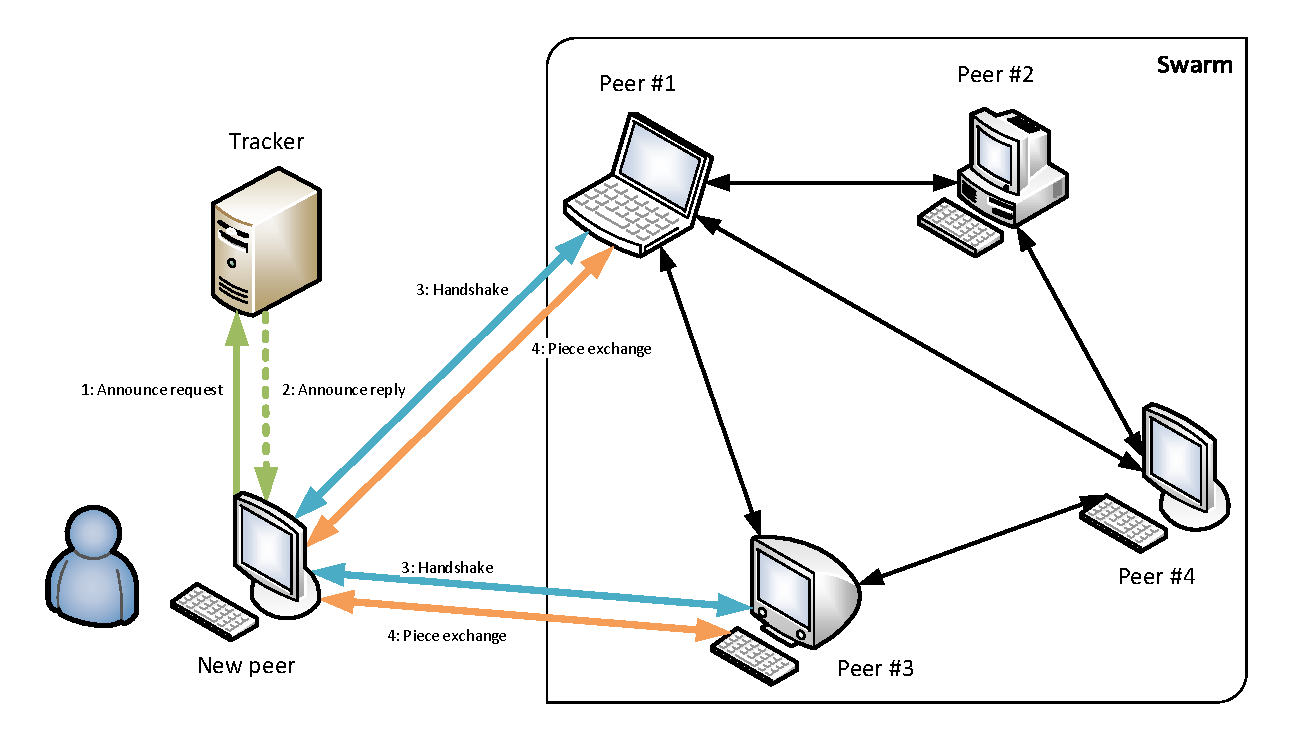
\includegraphics[width=\textwidth]{diagrams/bittorrent.pdf}
    \caption[BitTorrent architectural overview]{Overview of the BitTorrent architecture.}
    \label{fig:related:bittorrent}
\end{figure}

The client joins the swarm by sending an \emph{announce request} to the announce URL mentioned in the torrent metainfo file. The tracker receives this request, stores the new client's connection details and responds with an \emph{announce reply} containing a list of other peers with whom to connect. When other peers join the swarm, these stored connection details can be returned in their announce replies, inviting the new peers to connect with this client.

After retrieving a list of peers, the client opens \gls{TCP} connections with these peers. They both send a handshake message to ensure that both ends are indeed operating on the BitTorrent protocol and are trying to download the same torrent (identified by the metainfo hash).

After the handshake, the peers can start sending peer wire messages over the connection. The \texttt{have} and \texttt{bitfield} messages are used to notify about which pieces this peer has completely downloaded, so the other peer can potentially request them. The \texttt{request}, \texttt{piece} and \texttt{cancel} messages are used to transfer data of a single piece. This set of protocol messages is already sufficient to implement the file transfer. When a client has fully downloaded a piece, it sends a \texttt{have} message to all other peers so they are made aware of the newly available piece and may later \texttt{request} it. This continues until the client has downloaded every piece, at which point the client becomes a seed: there's nothing left to download, but it keeps uploading to help other peers in the swarm.

However, BitTorrent must also deal with limited network conditions and potentially `rogue' implementations of the protocol. \gls{TCP}'s congestion control performs poorly when sending over many connections at once, so not all opened connections should be used at the same time. Also, a `selfish' client implementation could ignore all received \texttt{request} messages, and only download from others without helping others by uploading to them. Therefore, BitTorrent clients maintain extra flags for every peer: the \emph{choke} flag means that the other end is not allowed to request data, and the \emph{interested} flag means that the other end would like to request data from this client. A peer sends \texttt{choke} or \texttt{unchoke} messages to notify whether this peer is choking the other end, and \texttt{interested} or \texttt{uninterested} messages to notify whether this peer is interested in one of the other's pieces. Clients can then use a choking algorithm to control which peers are allowed to download (by `unchoking' them), and which peers should be (temporarily) blocked (by `choking` them). For example, clients can keep only a limited number of connections unchoked, to prevent congestion. To promote `good behaviour' for clients, most BitTorrent implementations uses a \emph{tit-for-tat strategy} for their choking algorithm. With this strategy, peers will choke the other end when they are being choked (hence tit-for-tat), and will try to unchoke the other end when they are unchoked and the other end is interested.

\subsubsection{Advantages and disadvantages}
Every peer downloading missing pieces of the torrent's file also uploads the pieces it already has to other interested peers. This peer-to-peer file sharing approach has many advantages for both clients and distributors:
\begin{itemize}
\item Instead of having a single file server serving all clients wanting to download the file, BitTorrent employs the (often underused) upload capacity of those clients to help distributing the file to other clients. The combined upload capacity of these clients can be very large, and comes almost free to the distributor. The distributor only has to invest in a modest server acting as an initial seed, and letting the clients share the load.
\item Clients can download many pieces from many peers in parallel, which can lead to faster downloads.
\item BitTorrent is more failure-resilient than regular file distribution protocols such as \gls{FTP}. The \gls{FTP} server is a single point of failure: nobody can download the file if the server fails. In contrast, the failure of a single BitTorrent peer does not greatly impact the rest of the swarm. If every piece owned by the failed peer is still available at some other peer, all remaining peers can still download the full file. When the failed peer restarts, it also doesn't need to restart the complete download: it can verify the previously downloaded pieces using the checksums and resume downloading the missing pieces.
\item Regular file distribution protocols do not scale well when the number of simultaneously connected clients increases. \gls{FTP} requires 2 \gls{TCP} connections for each connected client trying to download a file, which can quickly consume the server's resources. The server also uses more upload bandwidth, which can cause congestion in the network. The classic solution to this involves installing more servers (`mirrors') in more locations, but this is expensive. In contrast, the load on the initial seed in BitTorrent actually \emph{decreases} as a torrent becomes more popular: all connected clients share the load to help others download the file.
\end{itemize}

However, there are also disadvantages to moving to peer-to-peer distribution:
\begin{itemize}
\item Unpopular torrents can become abandoned, with no active seeds in the swarm. This means that no new peers can download the full file, rendering the torrent useless until a seed is re-introduced. To prevent this, the distributor should maintain at least one seed in the torrent. This ensures that in the worst-case scenario, the whole file can be retrieved from the distributor's seed.
\item Moving the upload load from the distributor to the clients means that the networks of clients see more upload traffic. \glspl{ISP} optimize their consumer networks for `regular' consumer traffic behaviours, which consists primarily of download traffic. An \gls{ISP} might throttle torrent traffic in order to `shape' the traffic to a desired profile, reducing the performance of BitTorrent peers on its network.
\end{itemize}

\subsection{Local Peer Discovery for BitTorrent}
\label{sec:related:bt-ldp}
Local Peer Discovery is a BitTorrent protocol extension designed to support the local discovery of peers, aiming to maximize torrent traffic through the \gls{LAN} and reduce traffic through the \gls{ISP} \cite{bt-ldp}. Although there is no formal specification published as of the time of writing \footnote{Due to this lack of published specification, the only decent source \cite{bt-ldp} is on Wikipedia.}, it is quite consistently implemented in various BitTorrent clients and supports both \acrshort{IPv4} and \acrshort{IPv6} multicast.

The extension introduces a new discovery mechanism parallel to the centralized tracker, which uses \gls{UDP} messages periodically sent to a local multicast address to announce and discover peers in the local network. These messages are similar to standard announce requests, and include the torrent info hash and peer connection details. When other peers in the \gls{LAN} receive this multicast message, they can read the connection details and try to establish a peer connection.

Local Peer Discovery is not used very often in practice, as home user \glspl{LAN} are small and it is fairly uncommon to have many users downloading the same torrent inside the same local network. It makes much more sense in \glspl{WSN} where many peers do share the same local network, which is why this peer discovery mechanism is included in the protocol design (see \ref{sec:discovery:local}).

\section{Peer-to-peer distribution for WSNs}
\label{sec:related:wsn}

\subsection{Deluge}
\label{sec:related:deluge}
Deluge \cite{deluge} is a reliable data dissemination protocol for propagating large data objects from one or more source nodes to many other nodes in a \gls{WSN}. It allows incremental updates of large files to be efficiently flooded to the whole network.

Deluge assigns a monotonically increasing \emph{version number} to each new version of the distributed object, and subdivides the object into fixed-size pages. Since new versions often only have small difference compared to the previous version, many pages do not change between versions. Deluge uses this information to re-use pages from previous versions and prevent redundant page transfers. Every new page is identified by a monotonically increasing \emph{page number}.

Deluge nodes send periodic local broadcasts announcing their current version number and the latest available page (with the guarantee that all previous pages are also available). To control the transmission of potentially redundant announcements, Deluge uses the Trickle algorithm \cite{trickle} to do a `polite gossip'. For example, when a node hears a lot of its neighbours announcing the same version that it already has, it knows that there's no point in announcing its own version again. Most of its neighbours will probably already have heard one of the other neighbour's messages, so the node stays quiet to avoid broadcasting a redundant message.

\begin{figure}
    \centering
    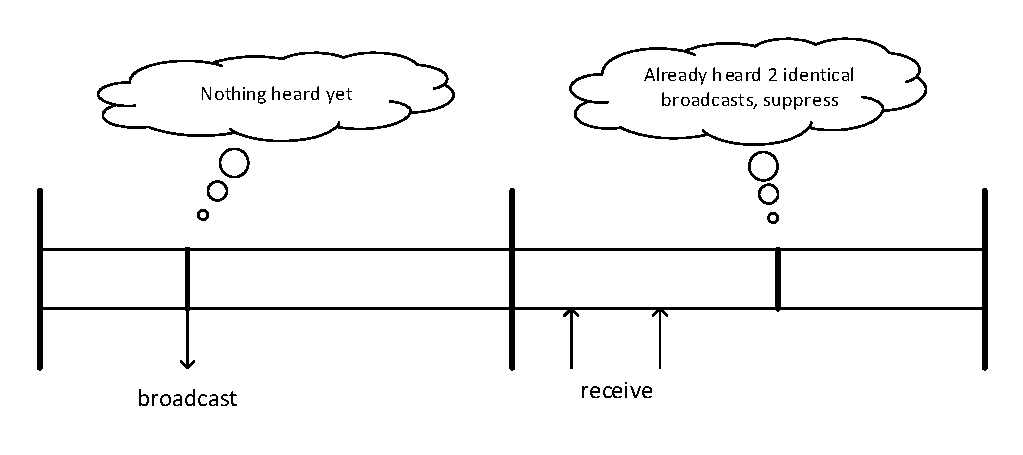
\includegraphics[width=\textwidth]{diagrams/trickle.pdf}
    \caption[Trickle algorithm example]{Example of Trickle's polite gossip algorithm. In the first interval, the node hasn't heard any other broadcasts yet and sends its broadcast. In the second interval, two identical broadcasts have already been received before the own broadcast is due, therefore the node suppresses its redundant broadcast.}
    \label{fig:related:trickle}
\end{figure}

Figure \ref{fig:related:trickle} shows an example of the Trickle algorithm in action. Before every interval, the node picks a random time $t \in [0, \tau]$ at which to schedule its own broadcast. If it doesn't hear a certain number of other identical broadcasts, it will send its broadcast at time $t$. If it does receive enough identical broadcasts, it will suppress its own broadcast at time $t$ and will not send anything during this interval. Because $t$ is randomly re-generated after every interval, the cost of sending broadcasts is distributed among all neighbours, ensuring that nodes use on average the same amount of energy for maintaining the announcements.

When a node hears one of its neighbours announcing a newer version number, it must update to the new version. Since many of its neighbours will hear this same announcement and likely also need to update, it would be wasteful for all these nodes to send requests to retrieve the new pages. Once again, Trickle is used to prevent redundant messages, so only a couple of nodes will send a broadcast to request the new page and only a few nodes will reply to the request. This allows new pages to propagate very efficiently throughout the network.

Deluge takes great advantage of local broadcasts in \glspl{WSN}, and makes flooding code updates very efficient. However, it assumes that all nodes in the network all need the same file, which might not be the case in heterogeneous deployments. NanoTorrent takes some advantage of local broadcasts by sending piece data as local multicasts (see \ref{sec:distrib:multicast}), however it can also use unicast messages to reach distant peers in a heterogeneous network.

\subsection{TinyTorrents}
\label{sec:related:tinytorrents}
TinyTorrents \cite{tinytorrents} is a peer-to-peer protocol designed for data dissemination in \glspl{WSN}. Like BitTorrent, TinyTorrents uses torrent files to describe the tracker's location and the file's contents. Peers join the swarm by contacting the tracker, and discover other peers with whom to connect and exchange data.

TinyTorrents recognizes that many of the problems BitTorrent tries to solve on the Internet also match the challenges posed by \glspl{WSN}. BitTorrent balances traffic load with its \gls{P2P} approach and avoids network partitions with a tracker. Data integrity is ensured with piece-wise checksums, and data replication is made efficient with its rarest-first piece selection policy. TinyTorrents adopts these design decisions, and similarly NanoTorrent follows the same reasoning.

However, BitTorrent's peer wire protocol consists of many short frequent messages such as \texttt{have}, \texttt{choke} and \texttt{interested} (explained in \ref{sec:related:bittorrent}). These are decremental for \gls{WSN} nodes, as they consume a lot of energy for transmission. TinyTorrents solves this by combining separate \texttt{have} messages into one less frequently sent \texttt{bitfield} message, and using a static approach based on the peer's position in the swarm to fairly distribute the load among \glspl{seeder} and \glspl{leecher}. NanoTorrent also drops BitTorrent's short \texttt{have} messages, but its tracker does not currently take fairness into account.

TinyTorrents supports interoperability with standard BitTorrent through a gateway acting as a bridge between the two protocols. The gateway can convert TinyTorrent torrents into BitTorrent torrents, allowing regular BitTorrent clients to download data from inside the \gls{WSN} and allowing \gls{WSN} nodes to download torrents published outside the \gls{WSN}. This allows remote users to access accumulated sensor measurements from the \gls{WSN}, or to reprogram nodes from anywhere on the Internet. NanoTorrent does not currently interoperate with BitTorrent, but can support interoperation with nodes on other \glspl{WSN} or the Internet thanks to its \gls{IPv6} foundation.

The authors of TinyTorrents recognize that their reliance on a centralized tracker is a weak point of their protocol, which is a single point of failure in their system. NanoTracker attempts to alleviate this by combining multiple peer discovery mechanisms, so peers can still discover each other even if the tracker (temporarily) becomes unavailable.

\section{Software evolution in WSNs}
\label{sec:related:evolution}

\subsection{Challenges and approaches for reprogramming WSNs}
Wang et al. \cite{wang-reprogramming} outline a framework to examine the different functions for a reprogramming solution for \glspl{WSN}, and survey the approaches taken by existing solutions.

Figure \ref{fig:related:wang-framework} shows their framework for reprogramming solutions. This includes features such as version control to manage different software versions, scope selection to control which nodes are affected by a reprogramming operation and code acquisition to request the download of a new version.

The authors note that \glspl{WSN} come with many challenges. The algorithms used on a \gls{WSN} node must be well designed to fit the constrained capacity profile of the node, they must be scalable and energy-efficient, and they must be able to handle unreliable communications.

The paper groups the approaches of various existing code dissemination protocols like Deluge by categories, such as the scope of an individual reprogramming operation, the ability to traverse a multi-hop network and the use of pipelining to accelerate the distribution. Although many protocols support multi-hop reprogramming, only a few such as Aqueduct and TinyCubus have support for a limited scope reprogramming.

Important objectives for a good reprogramming solution are reliability, scope coverage and autonomy: all targeted nodes must be able to autonomously and correctly retrieve the new software version. For practical usefulness, it must also be fast enough to cause minimal disruption to the normal operation of the \gls{WSN}, consume only a minimal amount of energy during the transmission and use only a minimal amount of \gls{RAM}.

In their framework, a \gls{P2P} file distribution protocol for \glspl{WSN} could fulfil the code acquisition and code dissemination functions of a network reprogramming solution. When a peer finds out that it should update to a new version, it can connect with the other peers with that same version and start exchanging the file with them.

\begin{figure}
    \centering
    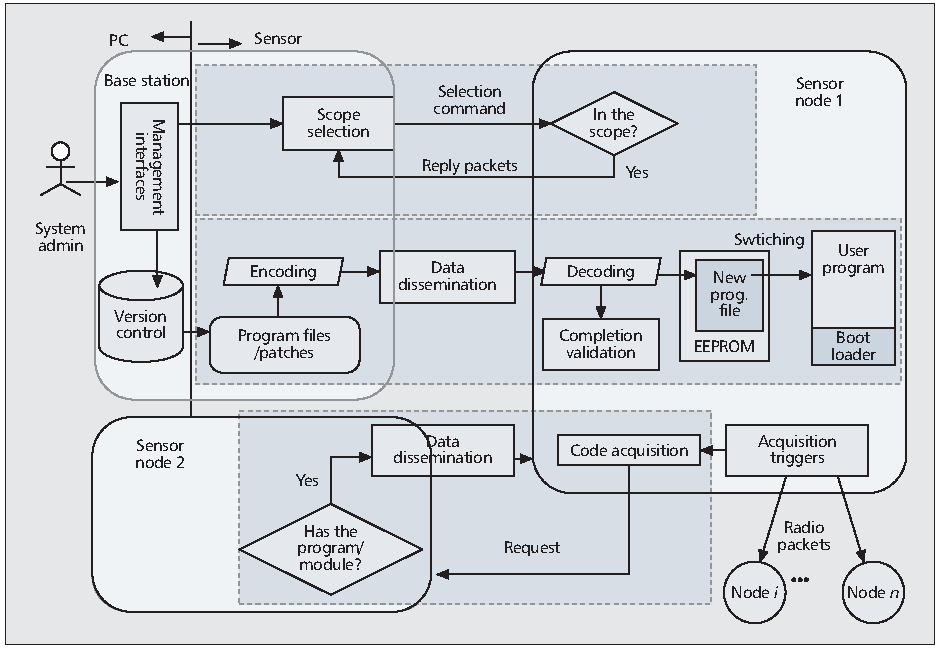
\includegraphics[width=\textwidth]{images/wang-reprogramming-framework.pdf}
    \caption[Framework for WSN reprogramming solutions]{Framework for WSN reprogramming solutions. \cite{wang-reprogramming}}
    \label{fig:related:wang-framework}
\end{figure}

\section{Critical discussion}
\label{sec:related:discussion}
BitTorrent has shown that \gls{P2P} file distribution can be made fast and easy-to-use on the Internet. It introduced a lot of good ideas, such as the choke/interested flags to control network load and punish misbehaving peers with a tit-for-that algorithm. However, these short frequent control messages can cause a lot of network traffic, which is the main cost factor for \gls{WSN} nodes. The design of a protocol aimed at \gls{WSN} nodes should be more careful with its transmissions.

BitTorrent Local Peer Discovery shows that multicast messages can be used to discover other peers on the same \gls{LAN} for faster local file distribution. However, multicast is not well supported in the current Internet infrastructures, many of which still use \gls{IPv4}. It is also very unlikely to have multiple BitTorrent clients on the same network downloading the same torrent, as consumer \glspl{LAN} are usually very small and corporate \glspl{LAN} mostly refrain from allowing BitTorrent traffic on their networks. This makes BitTorrent's Local Peer Discovery very underused on the Internet. However, the ideas behind its design are sound, and can be useful in the context of \glspl{WSN}.

There exist already a number of \gls{P2P} file transfer protocols for \glspl{WSN}. Deluge uses local broadcasts and listens for other neighbour's messages to prevent redundant transmissions. TinyTorrents is also influenced by BitTorrent's design, and even provides interopability with the original prototocol through the use of a gateway. However, none of these protocols leverage the \gls{IPv6} architecture which is becoming more common in \glspl{WSN} deployments as base for their communication. Deluge uses lower-level broadcasts for its communications, while TinyTorrents uses a custom TinyHop routing protocol. This opens an opportunity for a file distribution protocol which can run on top of the \gls{IPv6} network stack, allowing multi-hop connectivity between distant nodes in the network and even communication with outside networks.

A \gls{P2P} file distribution protocol for \glspl{WSN} could fulfil the code acquisition and code dissemination functions of a network reprogramming solution in the framework of Wang et al. \cite{wang-reprogramming}. Their paper also investigates protocols such as Trickle and Deluge, and notes that they only allow for full network reprogramming. There is an opportunity for a file distribution protocol that allows reprogramming of a limited scope of nodes, possibly with multiple reprogramming operations operating in parallel targeting different groups of nodes.
